\documentclass[12pt]{report}
% USER PACKAGE
\usepackage{graphicx}
\usepackage[italian]{babel}
\usepackage{hyperref}
\usepackage{subcaption}
\usepackage{float}
\usepackage{caption}
\usepackage{listings}
\usepackage{amsmath}
\usepackage[table]{xcolor}
\usepackage{pgfplots}
\usepackage{graphicx}
\usepackage{textcomp}


% OTHER SETTINGS
\hypersetup{colorlinks = true, urlcolor = blue}
\pagenumbering{gobble}
\usepackage{geometry}
\geometry{top = 3cm, bottom = 3cm,}
\pgfplotsset{compat=1.15}

% REMOVE 1ST PAGE----------------------------------------------
  %  \usepackage{atbegshi} % http://ctan.org/pkg/atbegshi 
  %  \AtBeginDocument{\AtBeginShipoutNext{\AtBeginShipoutDiscard}}
% -------------------------------------------------------------


\title{\textbf{Untitled Game} \\
    \large Relazione ESI Zephyr + Unity
    \begin{figure}[h!]
  \centering
  
\includegraphics[width=41mm]{img/home.png}
\end{figure}
}

\author{
        Giulio Zanchetta \\
        Department of Computer Science\\
        VR413626\\
            \and
        Giovanni Danieli\\
        Department of Computer Science\\
        VR408623\\
            \and
        Davide Benini\\
        Department of Computer Science\\
        VR409482
}

% BEGIN ---------------------------------------------------------
\begin{document}
\clearpage

\addtolength{\topmargin}{-15mm}
\thispagestyle{empty}
\date{}
\maketitle
\clearpage
\pagenumbering{arabic} % Arabic page numbers (and reset to 1)

\addtolength{\topmargin}{15mm}
\chapter{Introduzione}
\section{Installazione e utilizzo di Zephyr e di Unity}


Per iniziare abbiamo consultato il materiale on-line del software Zephyr e grazie ai tutorial messi a disposizione nel canale ufficiale di 3Dflow (\href{https://www.youtube.com/user/3DflowChannel}{3DflowChannel}) abbiamo appreso appieno l'utilizzo del software di fotogrammetria avanzata.


\subsection {Zephyr e ricostruzione tridimensionale}
Grazie a Zephyr \`e possibile ricostruire complessi elementi tridimensionali semplicemente scattando delle foto. \`E possibile poi esportare gli oggetti creati in vari formati il che da molta libert\`a per future modifiche con il software di modellazione pi\`u opportuno.
Come primo passo Zephyr analizza le immagini caricate per poi creare una nuvola di punti che coincide con i vertici dell'oggetto da creare, l'utente potr\`a poi decidere di addensare la nuvola di punti per poi applicargli una mesh e la texture.
Per iniziare abbiamo sperimentato l'utilizzo di diversi oggetti con diverse caratteristiche per capire come il software li analizzasse, abbiamo provato utilizzando oggetti di diversa altezza, spessore e diametro, abbiamo poi sperimentato le differenze in termini qualitativi con differenti quantit\`a di immagini per capire quale fosse il numero minimo necessario per riscontrare un risultato di buona qualit\`a per oggetti di piccole dimensioni (quali tazze o libri) individuando che per un buon risultato sono neccessarie almeno 30 fotografie.

\begin{figure}[H]
  \centering
  \begin{subfigure}[b]{0.365\linewidth}
    \centering
    \includegraphics[width=\linewidth]{img/pianta1.JPG}
    \caption{Oggetto reale da ricostruire.}
  \end{subfigure}
  \begin{subfigure}[b]{0.4\linewidth}
    \centering
    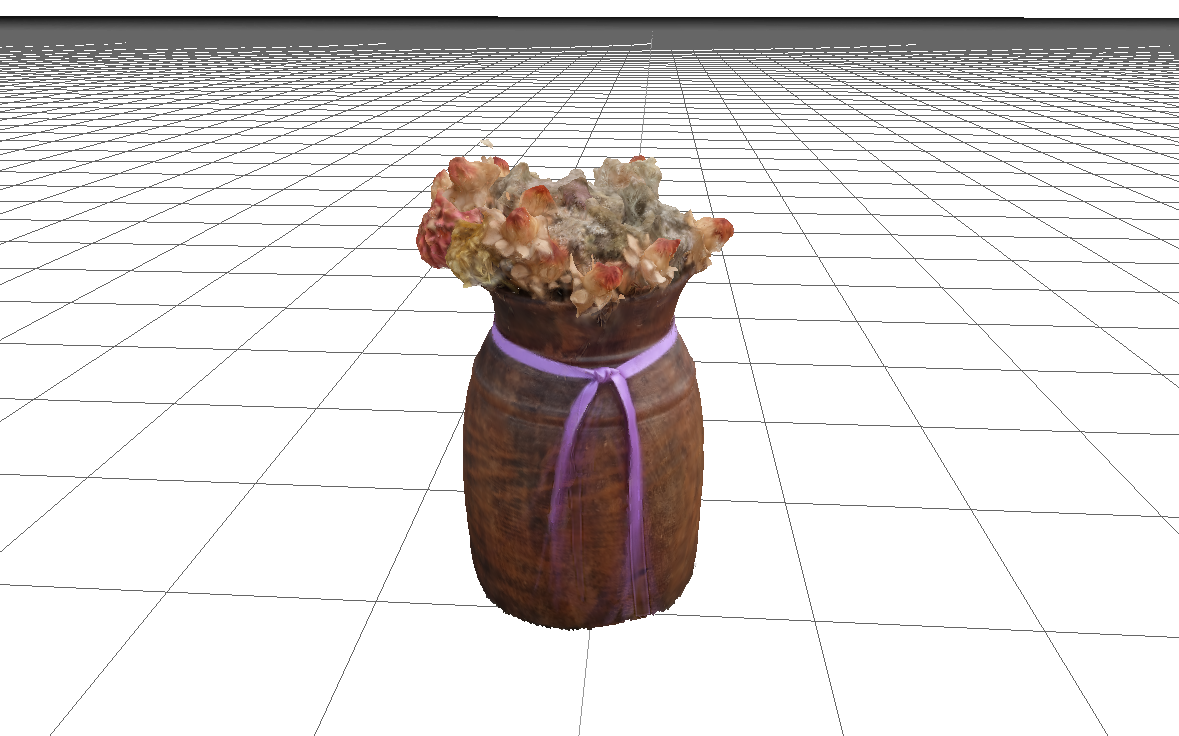
\includegraphics[width=\linewidth]{img/pianta.png}
    \caption{Oggetto ricostruito da Zephyr.}
  \end{subfigure}
  \captionsetup{justification=centering}
  \caption{Un vaso di fiori (40 foto); nonostante il basso livello di contrasto fra i fiori e lo sfondo zephyr ha ricreato l'oggetto egregiamente}
\end{figure}
Abbiamo successivamente utilizzato i tool per il mascheramento e la modifica degli oggetti messi a disposizione dal software Zephyr per capire come effettuare delle semplici modifiche senza dover ricorrere ad altri software.
Questi strumenti servono principalmente per rimuovere eventuali sfondi o punti d'appoggio dall'oggetto creato.
\begin{figure}[H]
  \centering
  \begin{subfigure}[b]{0.37\linewidth}
    \centering
    \includegraphics[width=\linewidth]{img/coltello1.JPG}
    \caption{Oggetto reale da ricostruire.}
  \end{subfigure}
  \begin{subfigure}[b]{0.4\linewidth}
    \centering
    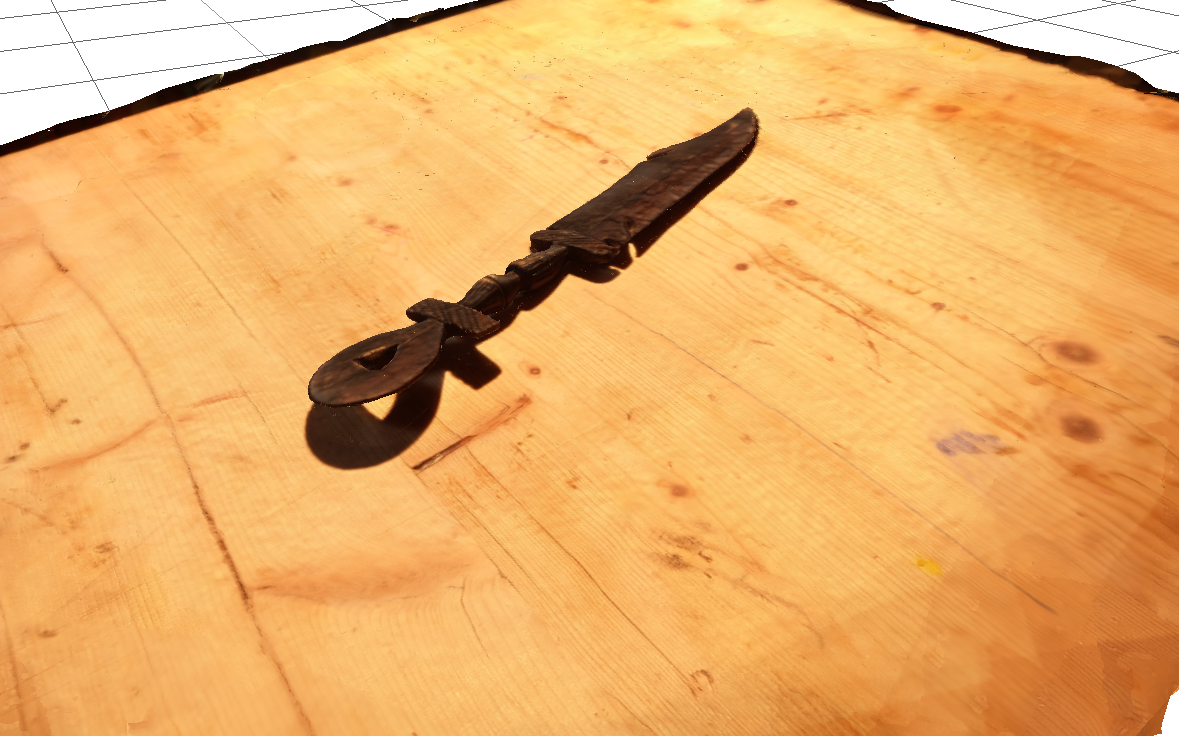
\includegraphics[width=\linewidth]{img/coltello.png}
    \caption{Oggetto ricostruito da Zephyr.}
  \end{subfigure}
  \captionsetup{justification=centering}
  \caption{Un coltello apribuste (50 foto), malgrado il lieve spessore la ricostruzione ha mantenuto fede ai dettagli}
\end{figure}

Ci siamo poi spinti oltre mettendo alla prova le capacit\`a di Zephyr di ricostruire elementi tridimensionali partendo da immagini con rumore gaussiano e successivamente elaborate con matlab per ridurre il suddetto rumore.

Per iniziare abbiamo scattato le foto in una stanza buia con ISO pari a 25.600 per ricreare un rumore gaussiano senza per\`o ottenere il risultato sperato (probabilmente la macchina fotografica, Fujifilm X-T1, ha applicato in modo automatico un filtro antirumore) cos\`i abbiamo creato un filtro passa basso ideale con matlab:

\begin{equation}
H(u,v) = 
\begin{cases}
1,se D(u,v)\leq D_0
\\
0,se D(u,v)>D_0
\end{cases}
\end{equation}

\begin{equation}
D(u,v) = \sqrt{(u-M/2)^{2}) + (v-N/2)^{2})}   
\end{equation}
\newpage
 \noindent ottenendo il seguente risultato

\begin{figure}[H]
  \centering
  \begin{subfigure}[b]{0.45\linewidth}
    \centering
    \includegraphics[width=\linewidth]{img/pentola/original_noised.png}
    \caption{Immagine originale.}
  \end{subfigure}
  \begin{subfigure}[b]{0.45\linewidth}
    \centering
    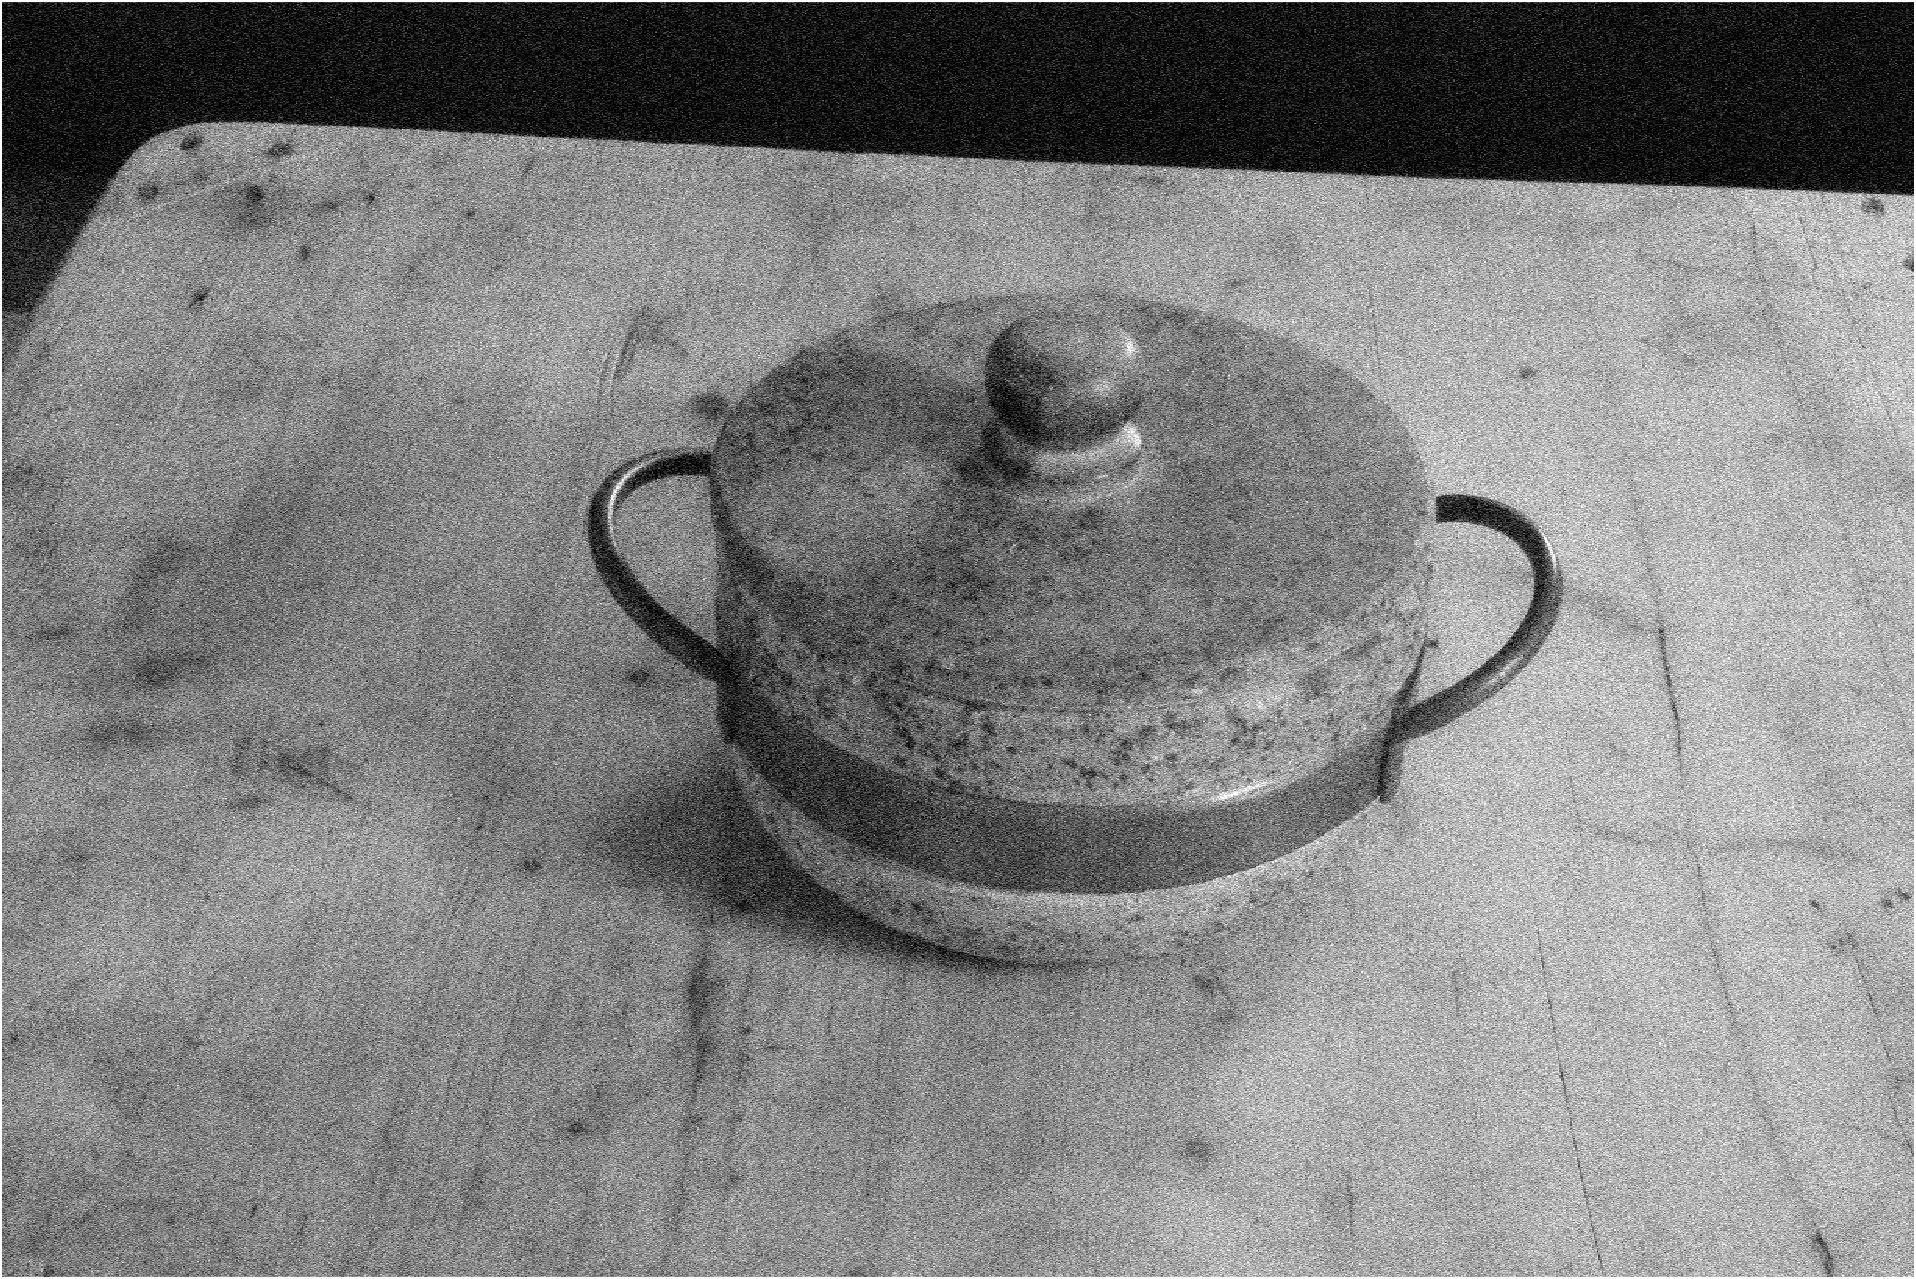
\includegraphics[width=\linewidth]{img/pentola/noised_image.png}
    \caption{Dopo aver applicato il rumore.}
  \end{subfigure}
\end{figure}

Abbiamo poi tolto il rumore generato grazie a matlab e deep learning ottenendo un risultato quasi pari all'originale. Per far ci\`o abbiamo però dovuto convertire l'immagine da RGB a scala di grigi.

\textit{net = denoisingNetwork('DnCNN');\\denoisedI = denoiseImage(noisyI, net);\\figure\\imshow(denoisedI)\\title('Denoised Image')\\imwrite();}

Abbiamo scelto questo procedimento perch\'e \`e stato quello che ha dato i risultati migliori.
%ORIGINALE -NOISED- DENOISED
\begin{figure}[H]
  \centering
  \begin{subfigure}[b]{0.4\linewidth}
    \centering
    \includegraphics[width=\linewidth]{img/pentola/original_noised.png}
    \caption{Immagine originale.}
  \end{subfigure}
  \begin{subfigure}[b]{0.4\linewidth}
    \centering
    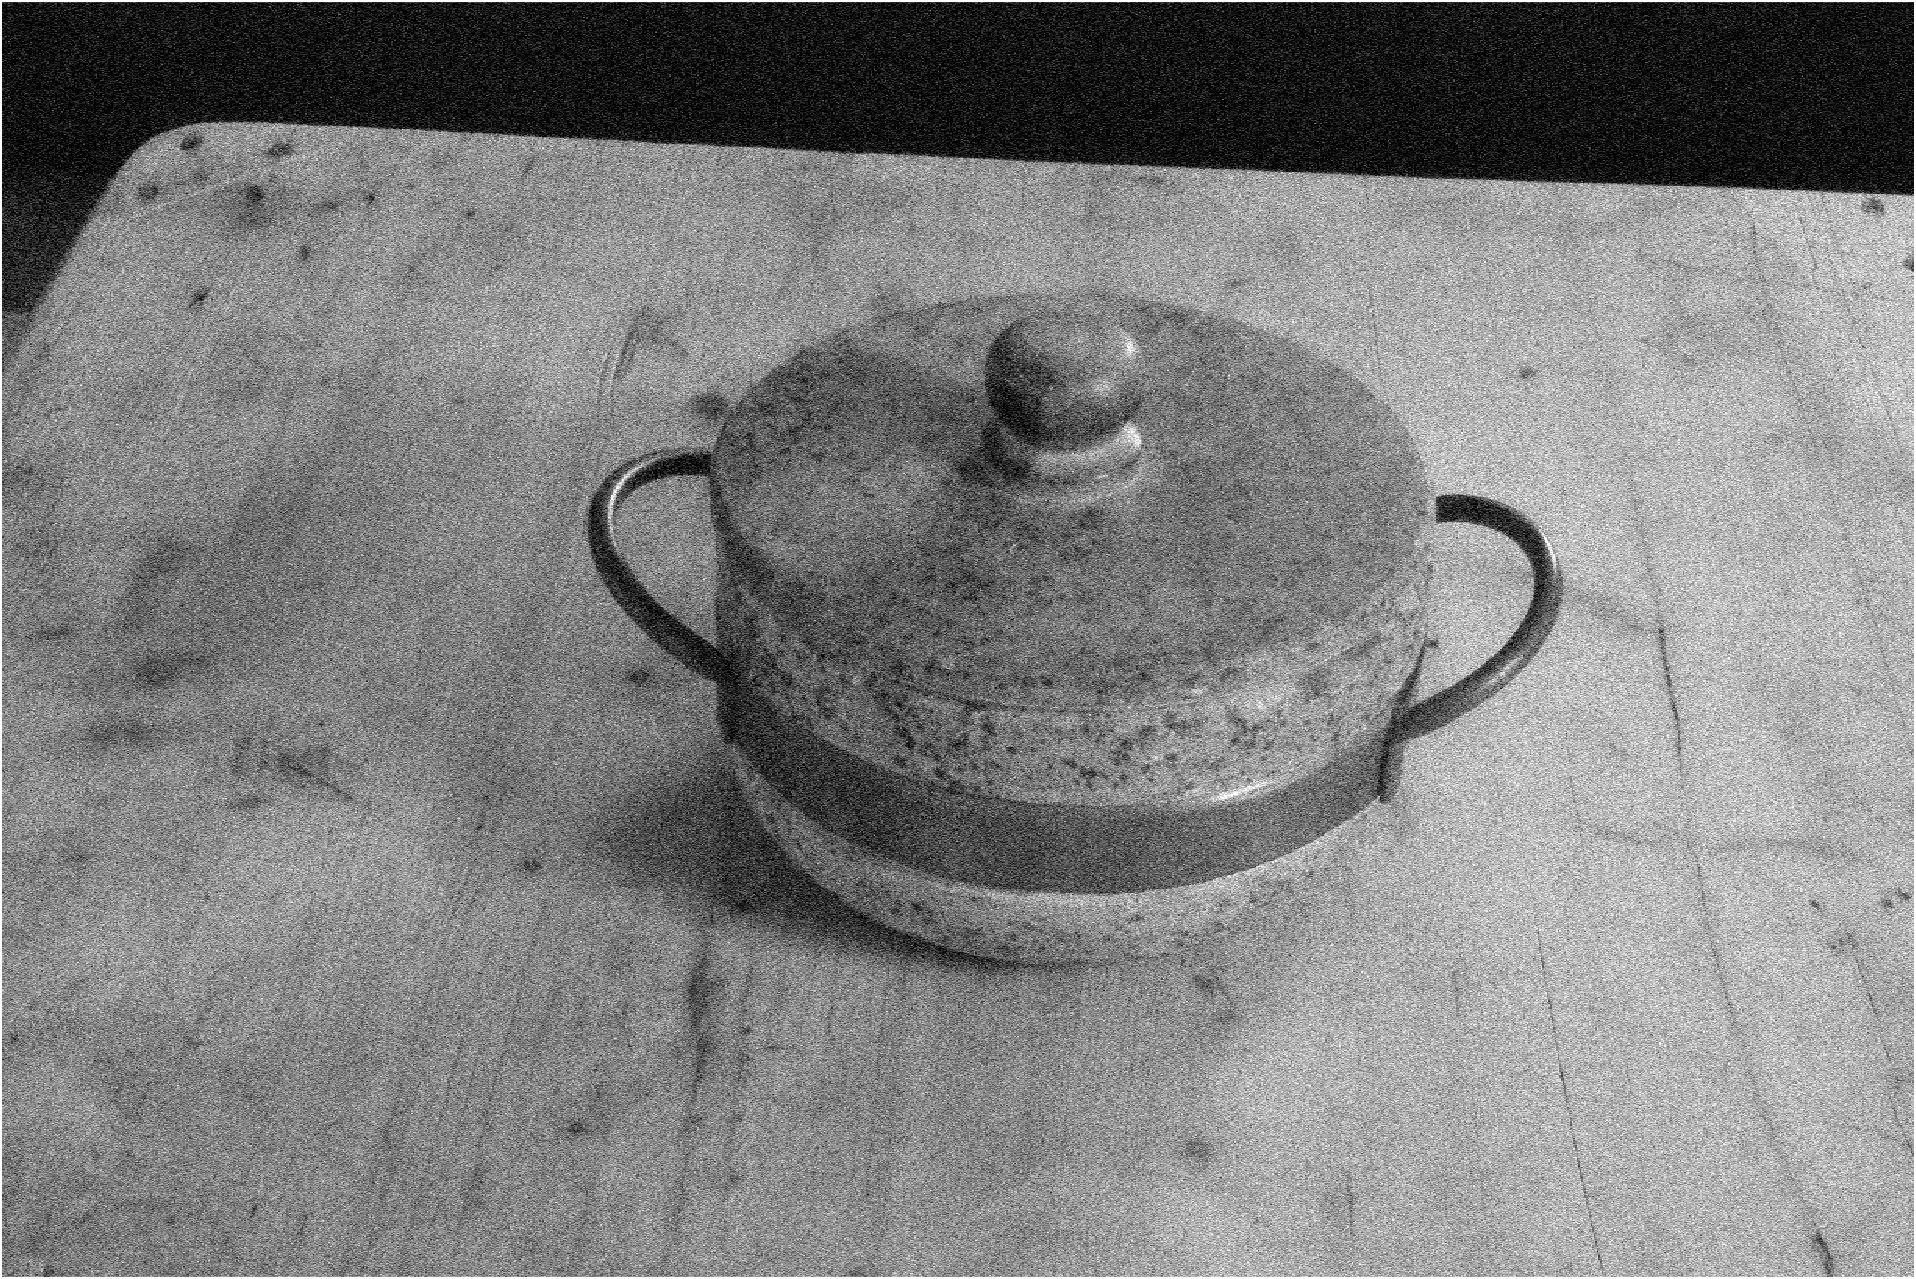
\includegraphics[width=\linewidth]{img/pentola/noised_image.png}
    \caption{Dopo aver applicato il rumore.}
  \end{subfigure}
  \begin{subfigure}[b]{0.6\linewidth}
    \centering
    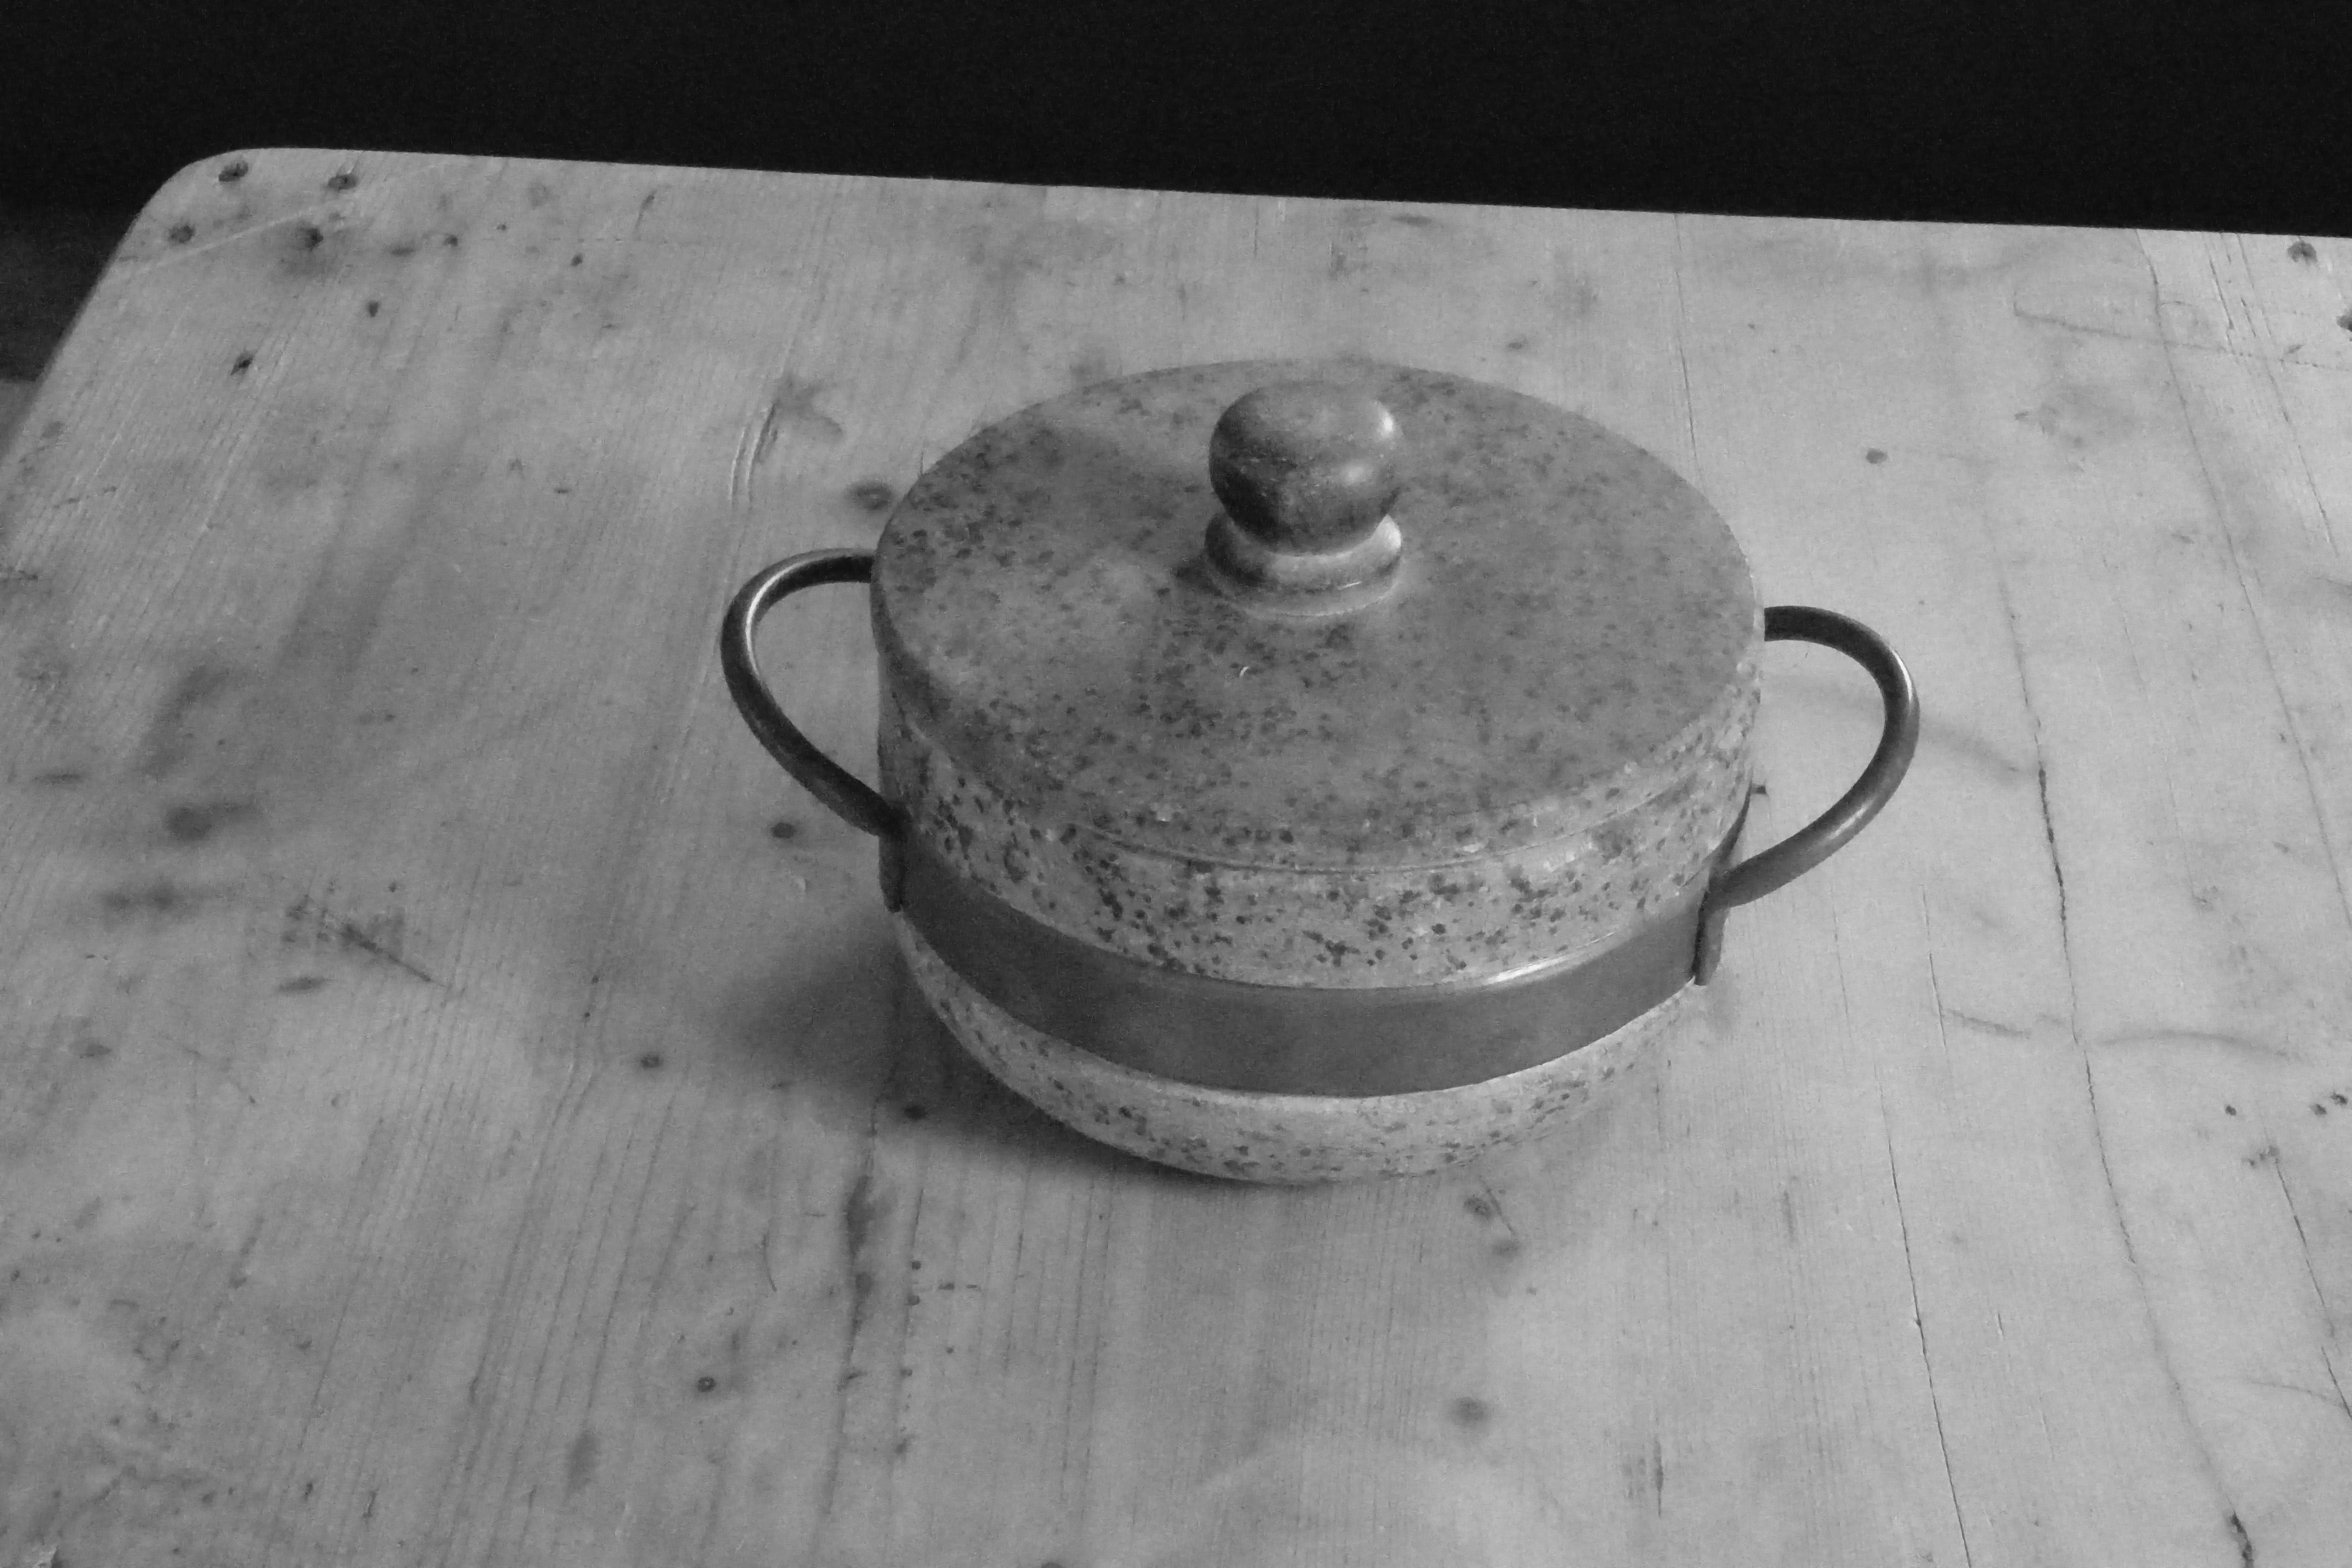
\includegraphics[width=\linewidth]{img/pentola/denoised_AI.jpg}
    \caption{Dopo aver tolto il rumore con MatLab}
  \end{subfigure}
\end{figure}

Abbiamo poi provato a sistemare un immagine fuori fuoco grazie all'algoritmo di convoluzione per rimuovere il blur dall'immagine:


\begin{equation}
f_1 * f_2 (t)  =  \int_{-\infty}^{\infty}{f_1(\tau)f_2 (t - \tau)d\tau}
\end{equation}

%BLURRED IMAGE - DEBLURRED IMAGE

\begin{figure}[H]
  \centering
  \begin{subfigure}[b]{0.35\linewidth}
    \centering
    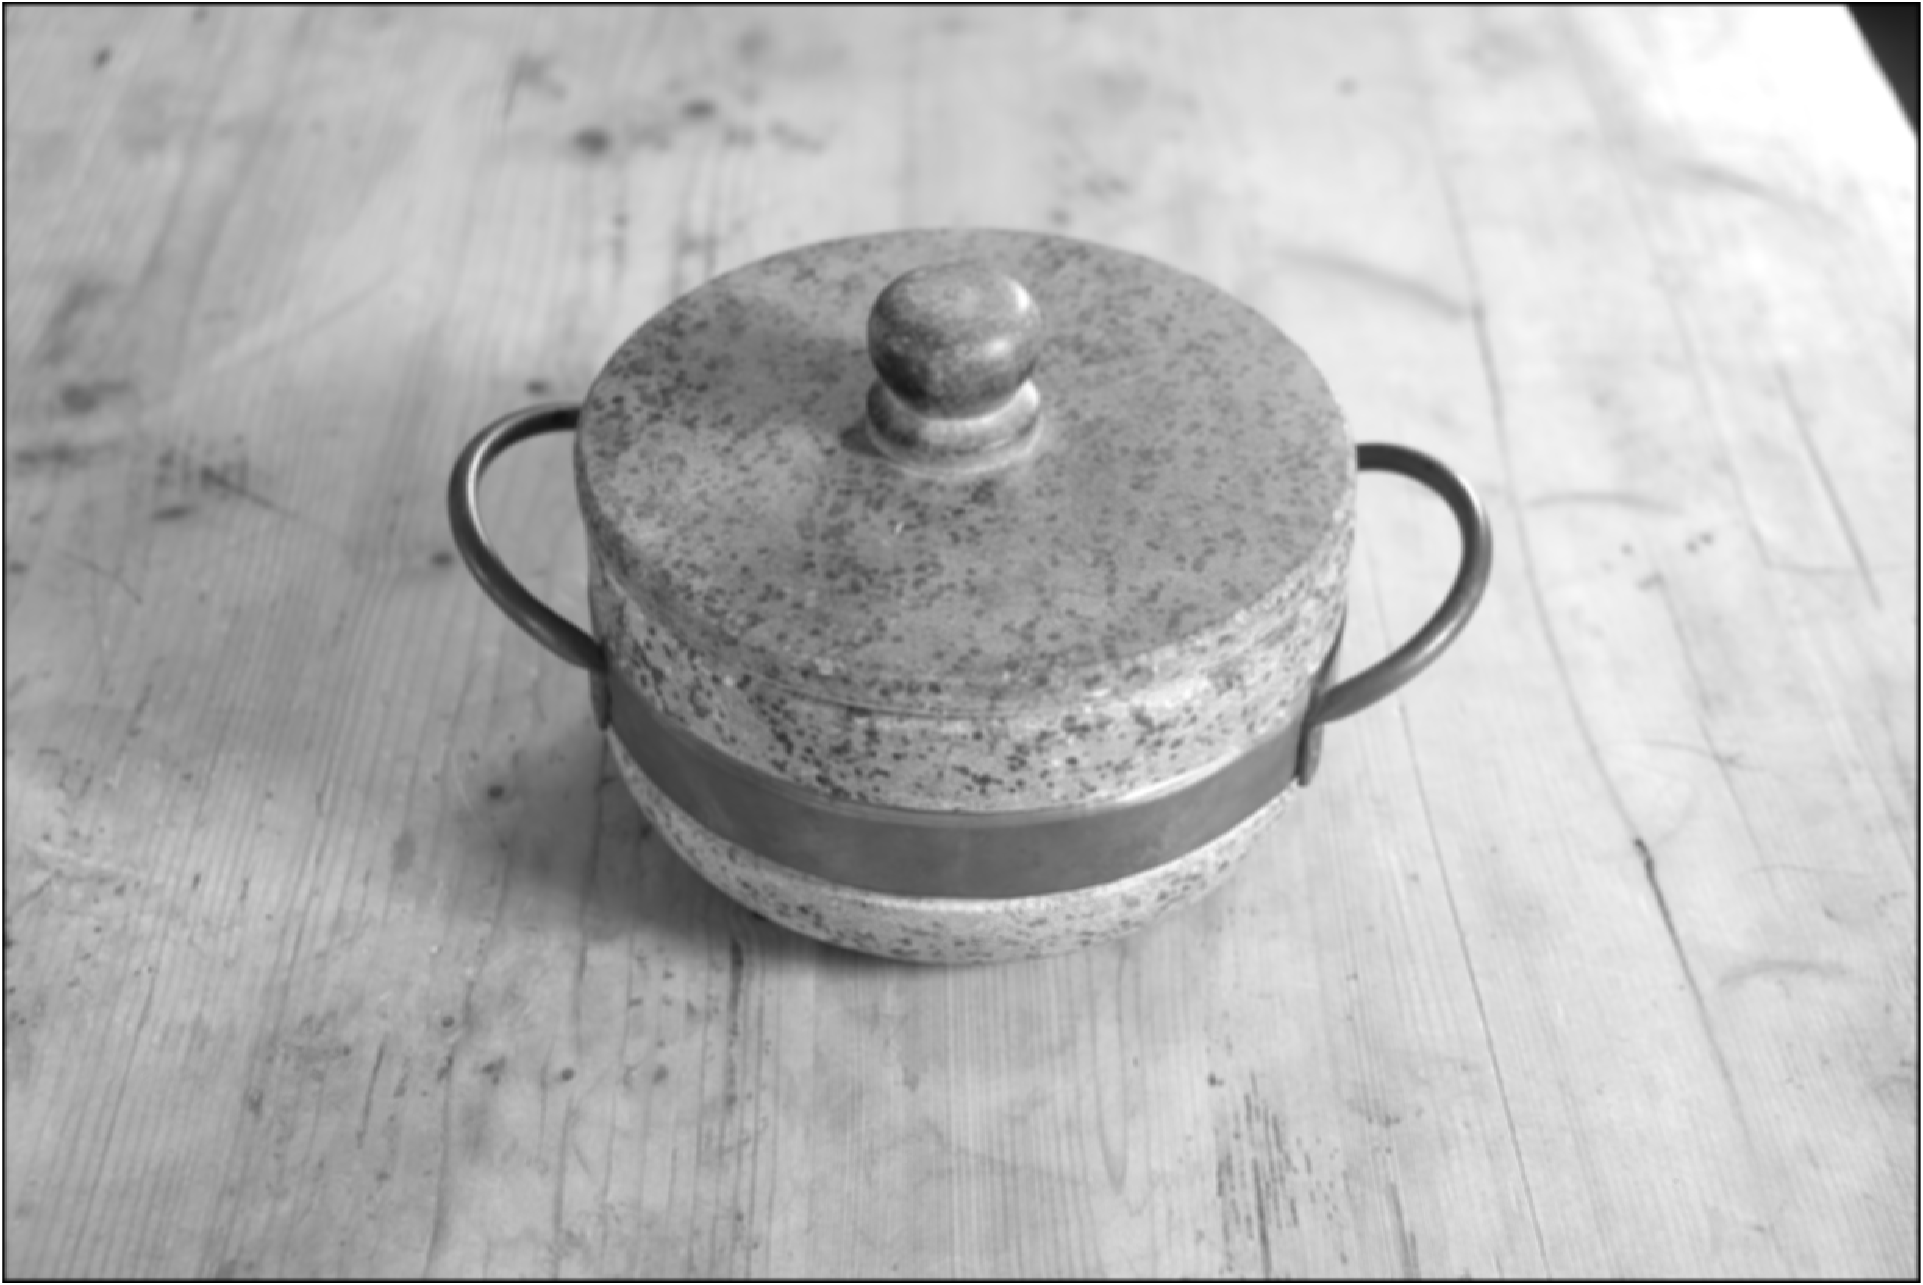
\includegraphics[width=\linewidth]{img/pentola/blurred_deconv.png}
    \caption{Immagine sfocata.}
  \end{subfigure}
  \begin{subfigure}[b]{0.35\linewidth}
    \centering
    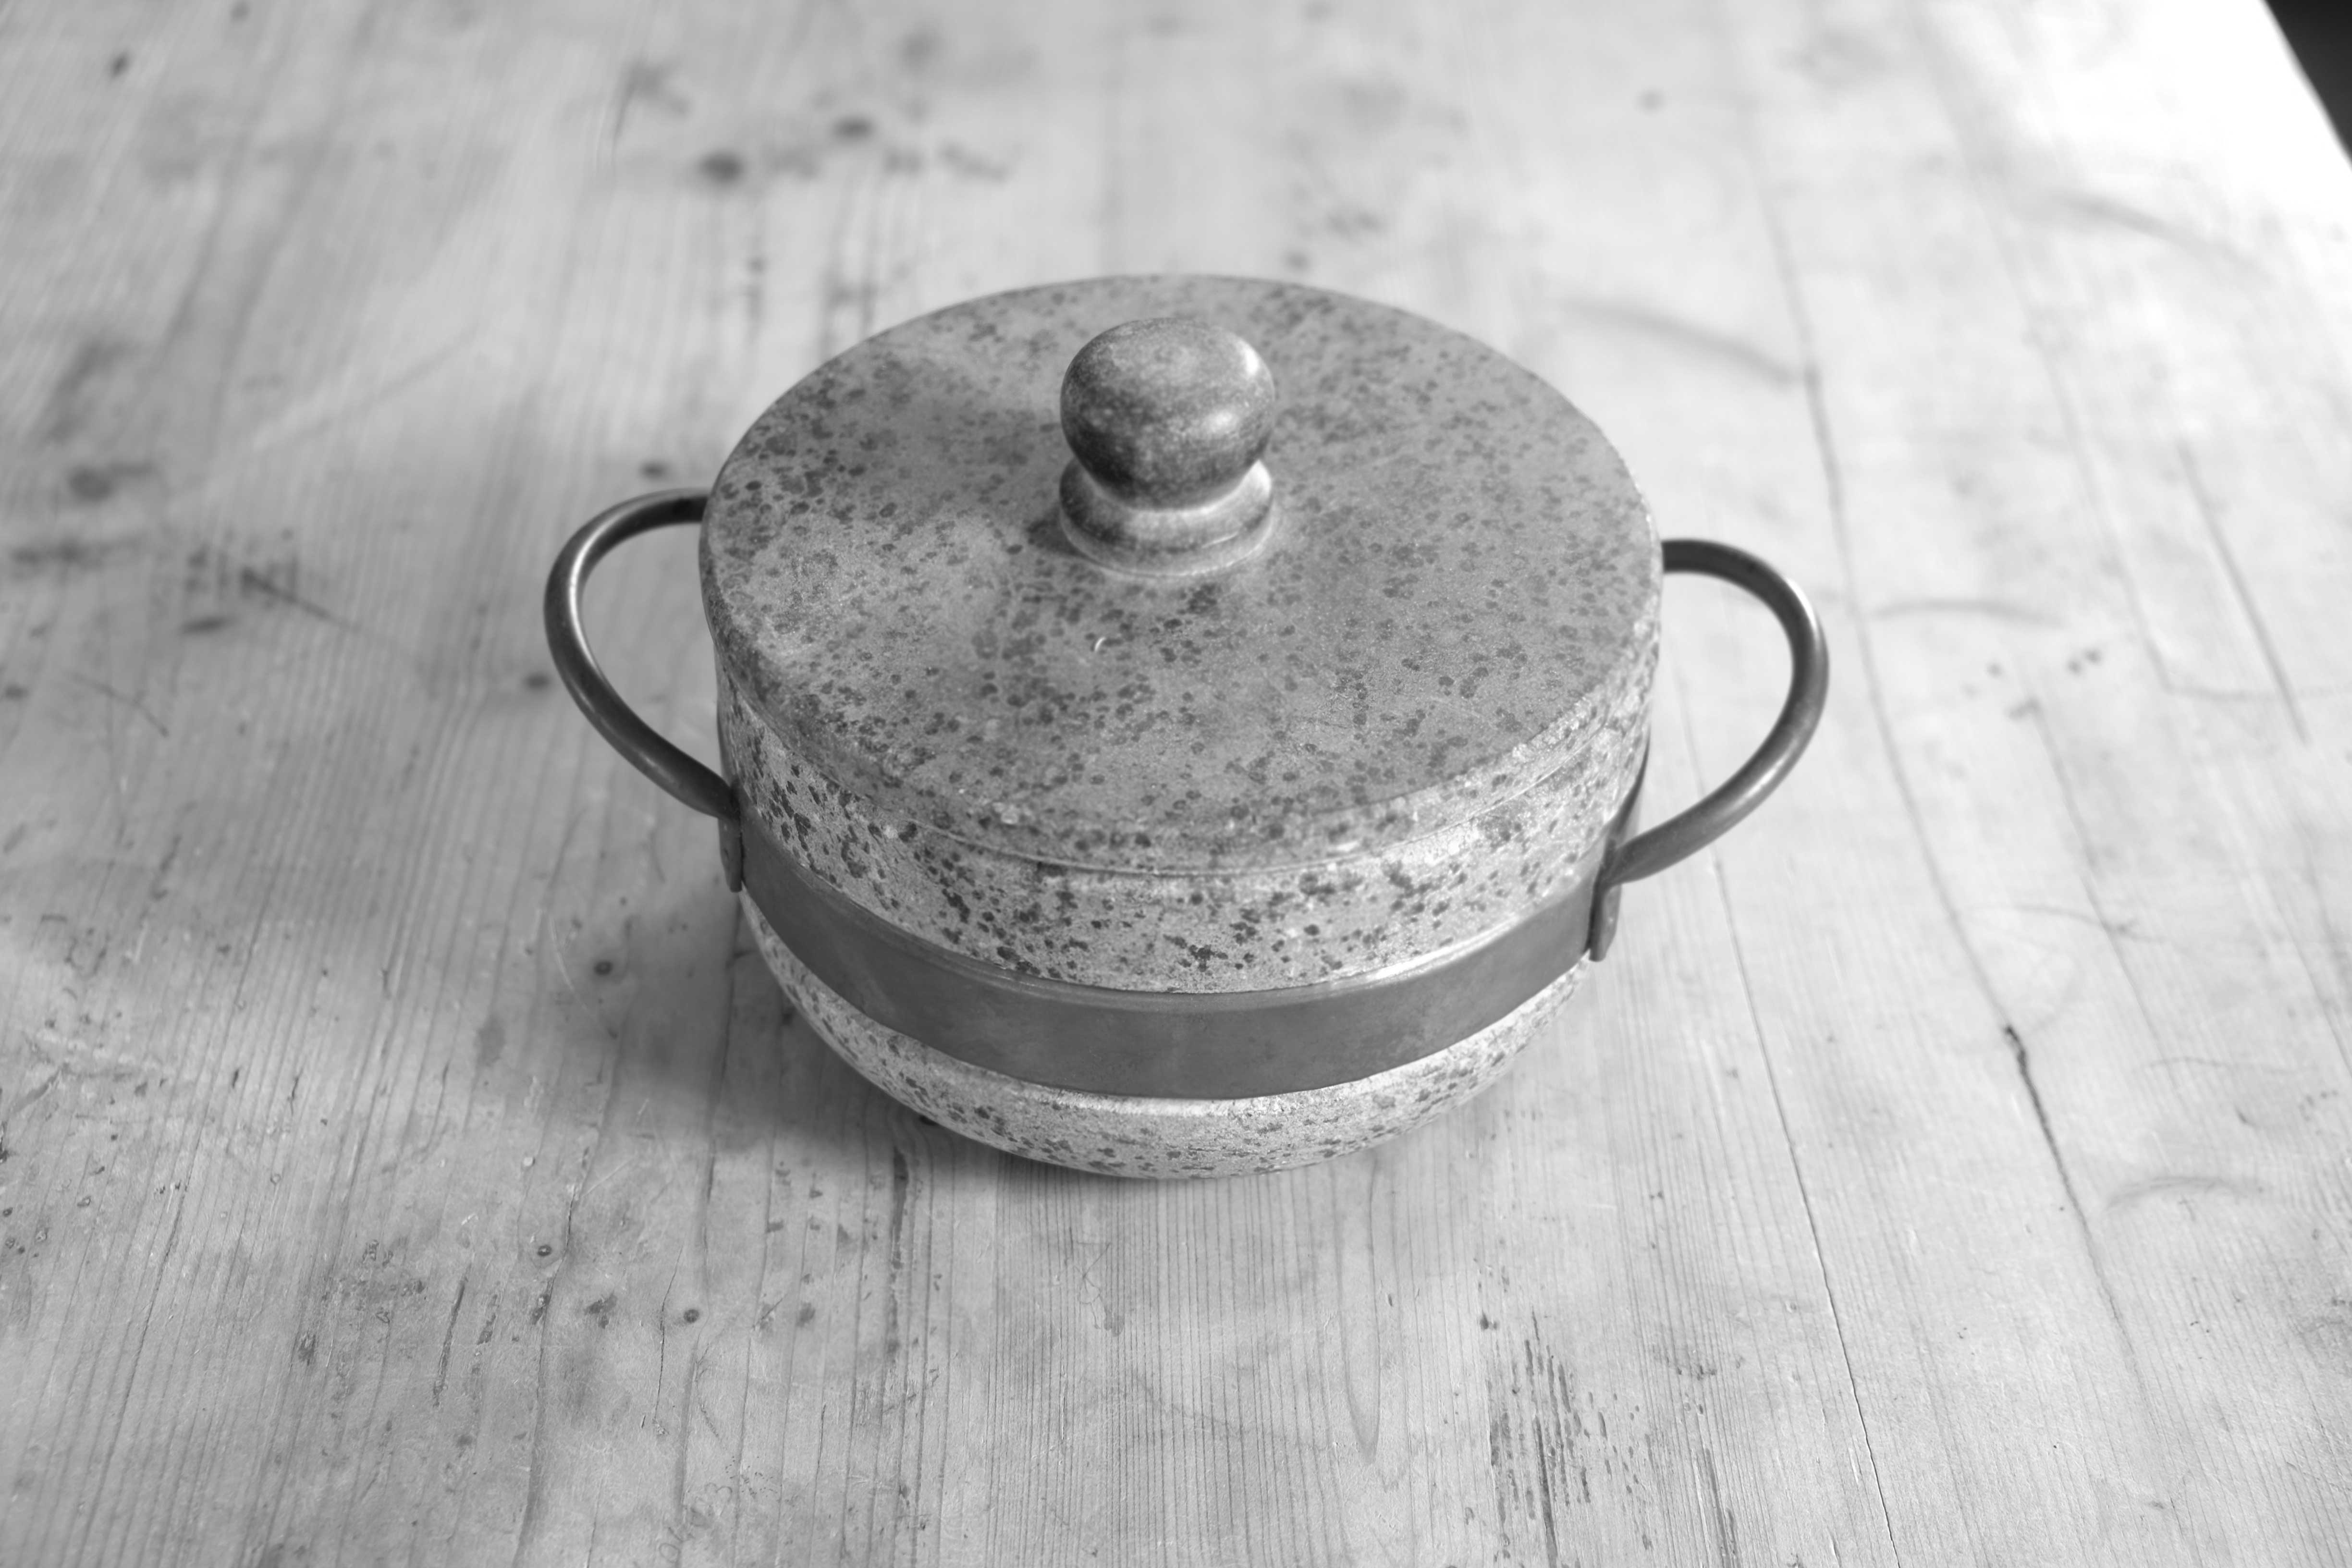
\includegraphics[width=\linewidth]{img/pentola/afuoco.jpg} %Sostituire
    \caption{Dopo l'algoritmo.}
  \end{subfigure}
\end{figure}

Infine abbiamo utilizzato le immagini restaurate per creare i modelli con zephyr ricavando dei risulati soddisfacenti. Nel caso della rimozione del rumore, trascurando la perdita del colore, l'oggetto ottenuto ha un qualit\`a quasi pari all'originale. Nel caso del blur la differenza sul pdf \`e meno percettibile ma si può comunque notare una riduzione della sfocatura.
%CONTINUA----------------------------------------------------------------

%OGGETTO ZEPHYR - OGGETTO GRAYSCALE DENOISED - GRAYSCALE DEBLURRED



\begin{figure}[H]
  \centering
  \begin{subfigure}[b]{0.45\linewidth}
    \centering
    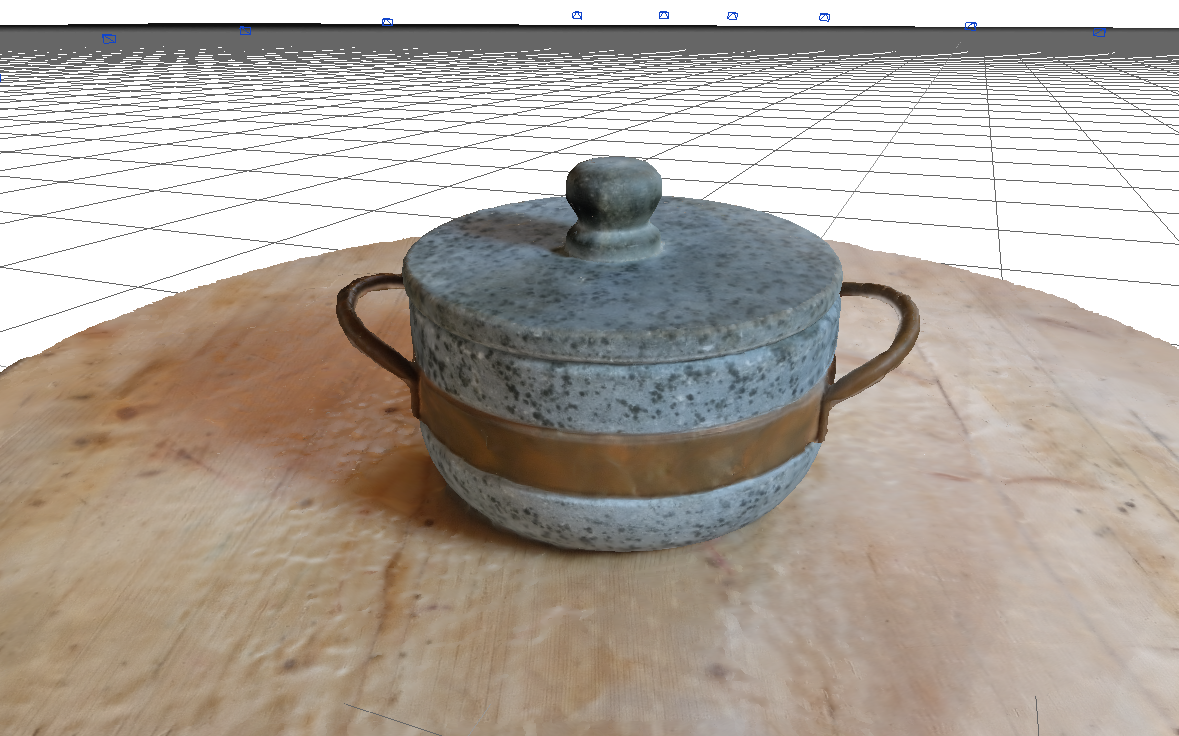
\includegraphics[width=\linewidth]{img/pentola/oggetto.png}
    \captionsetup{justification=centering}
    \caption{Oggetto reale ricostruito senza applicazione di filtri.} %sostituire
  \end{subfigure}
   \begin{subfigure}[b]{0.45\linewidth}
    \centering
    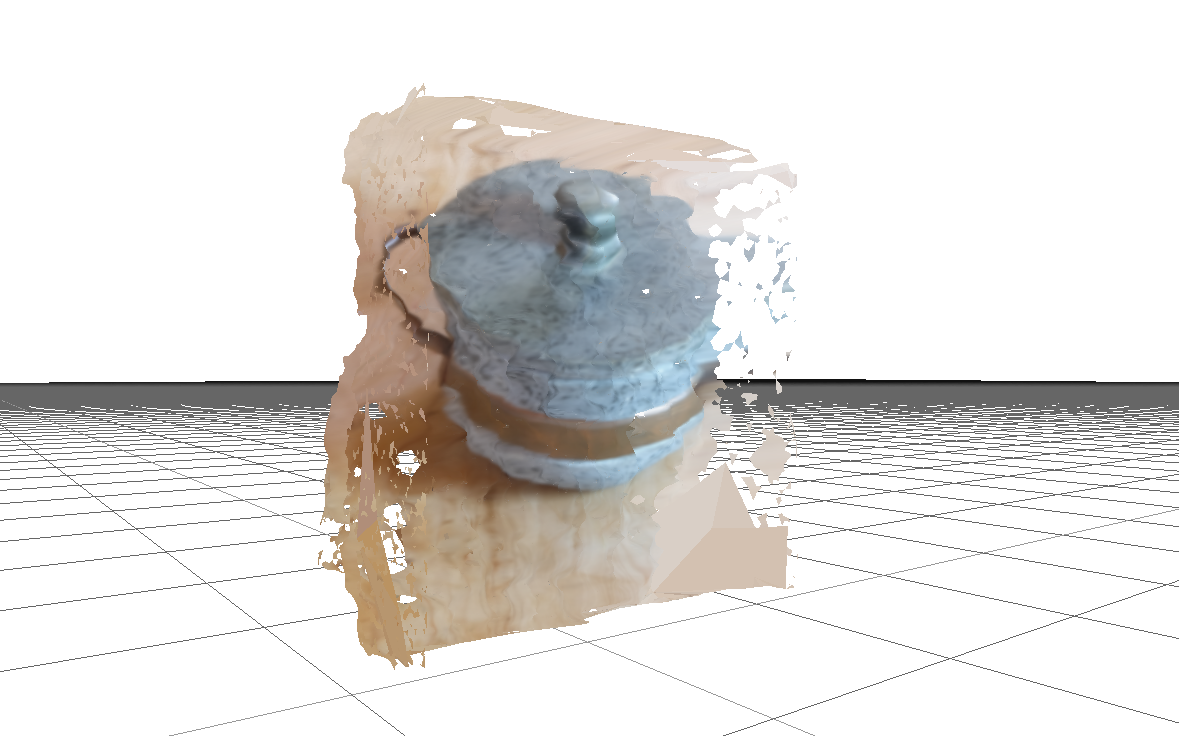
\includegraphics[width=\linewidth]{img/pentola/oggetto_blurred.png}
    \captionsetup{justification=centering}
    \caption{Oggetto ricostruito da immagini con rumore senza rinforzo.}
  \end{subfigure}
  \begin{subfigure}[b]{0.45\linewidth}
    \centering
    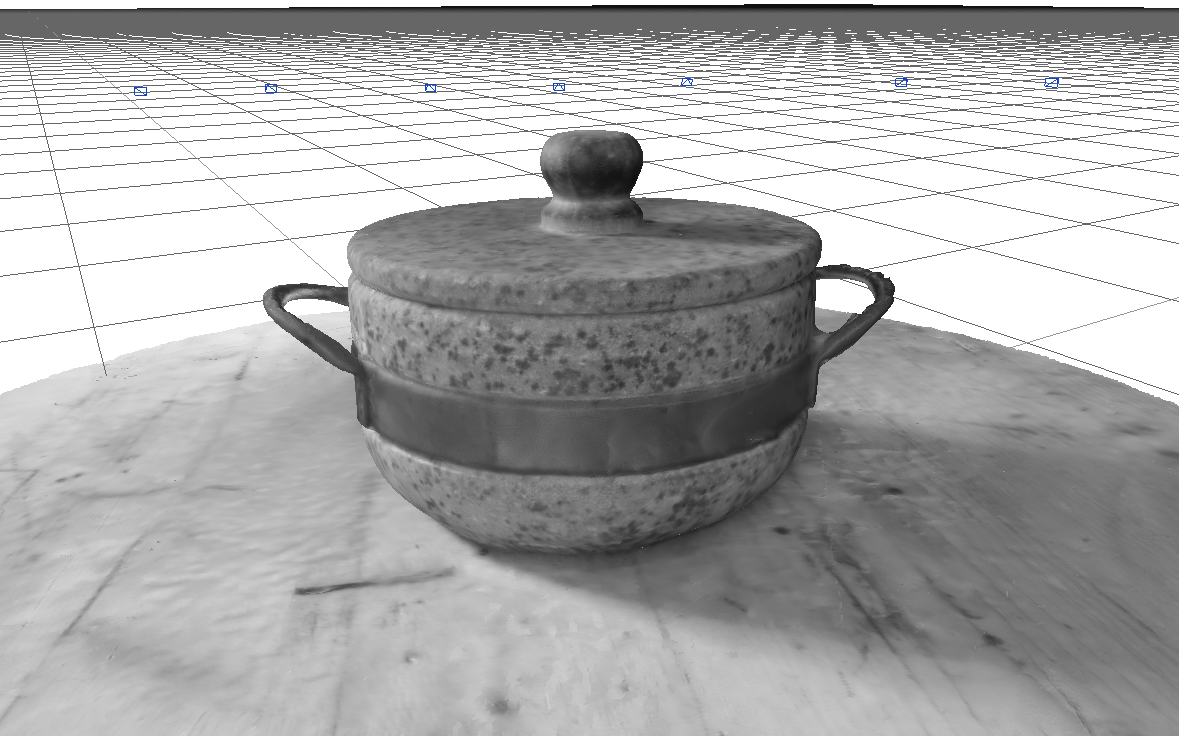
\includegraphics[width=\linewidth]{img/pentola/oggetto_grayscale.png} %sostituire
    \captionsetup{justification=centering}
    \caption{Oggetto ricostruito da immagini a cui \`e stato rimosso il rumore.}
  \end{subfigure}
  \begin{subfigure}[b]{0.45\linewidth}
    \centering
    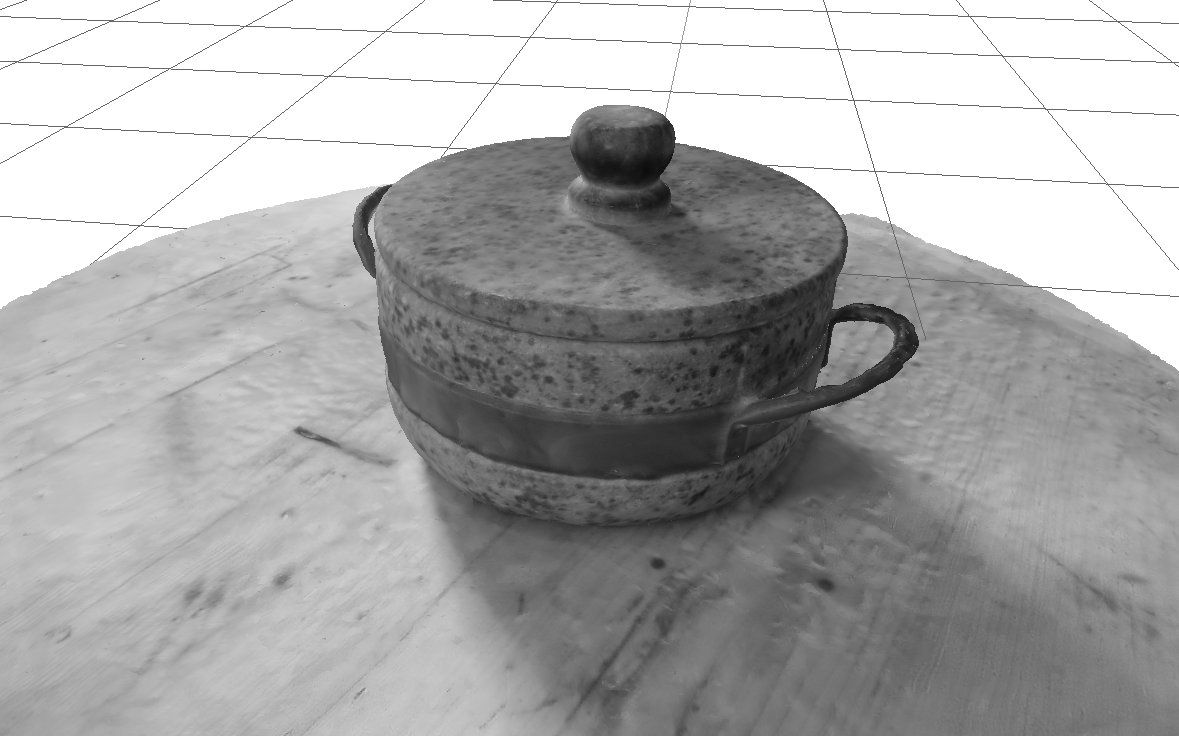
\includegraphics[width=\linewidth]{img/pentola/oggetto_deblurred.png}
    \captionsetup{justification=centering}
    \caption{Oggetto ricostruito da immagini a cui \`e stato rimosso il blur.}
  \end{subfigure}
  \captionsetup{justification=centering}
  \caption{Pentola (64 immagini), nel caso della ricostruzione con le immagini senza rinforzo zephyr non \`e riuscito ad elaborare tutte le immagine o parzialmente ed \`e stato ottenuto un risultato scadente, recuperato poi con il rinforzo delle immagini su matlab}
\end{figure}

\newpage
\subsection{Model Processing}
Il processo di costruzione delle immagini per ricreare un oggetto adatto al funzionamento all'interno di un motore grafico  \`e composto da vari processi.
% Inserire grafico con processo produzione oggetto completo adatto ad essere inserito su un motore grafico
Nella prima parte bisogna decidere il software con il quale ricostruire il set di foto che  \`e stato acquisito. Per fare ci\`o bisogna assicurarsi che ogni foto all'interno del set abbia i requisiti per ricostruire un modello di buona qualit\`a; bisogna escludere quindi le immagini con esposizione troppo bassa o troppo alta, immagini mosse o sgranate perch\`e potrebbero andare a peggiorare un risultato potenzialmente buono, \`e meglio avere 100 foto buone che  700 di buone e 100 di cattive nello stesso photoset.
% ultima frase di riscrivere
Se le immagini sono state catturate in formato RAW \`e necessario convertirle in un formato che sia adatto al programma di ricostruzione, per mantenere la miglior qualit\`a \`e consigliato convertirle nel formato TIFF.
\newline
\newline
Successivamente bisogna bilanciare le immagini acquisite, per questo si pu\`o utilizzare "Camera RAW" di Adobe oppure "DC RAW", un programma open-source creato da Dave Coffin.
\newline
\newline
Bisogna quindi convertire le immagini da 32 bit a 8 bit, questo per evitare problemi con la correzione di gamma all'interno del software di ricostruzione; in ogni caso la maggior parte dei software di ricostruzione converte in automatico le immagini a 8 bit, per cui non vi \`e perdita di informazioni.
\newline
\newline

% Paragrafo informazione oggetto e perche e' stato scelto 

Per costruire l'oggetto principale della scena abbiamo utilizzato il software "Zephyr" di 3DFlow.
Aperto il programma abbiamo importato il nostro set di immagini (composto da 350 elementi), a questo punto
%migliorare frase sotto
abbiamo calcolato la nuvola di punti sparsa, la nuvola di punti densa, la mesh e la texture. Una volta calcolato il modello abbiamo esportato le mesh, una ad alta risoluzione ed una a bassa, che utilizzeremo come sorgenti per il baking delle normali. Abbiamo poi importato alla fine le mesh nel programma "3DSMax".
\begin{figure}[H]
    \centering
    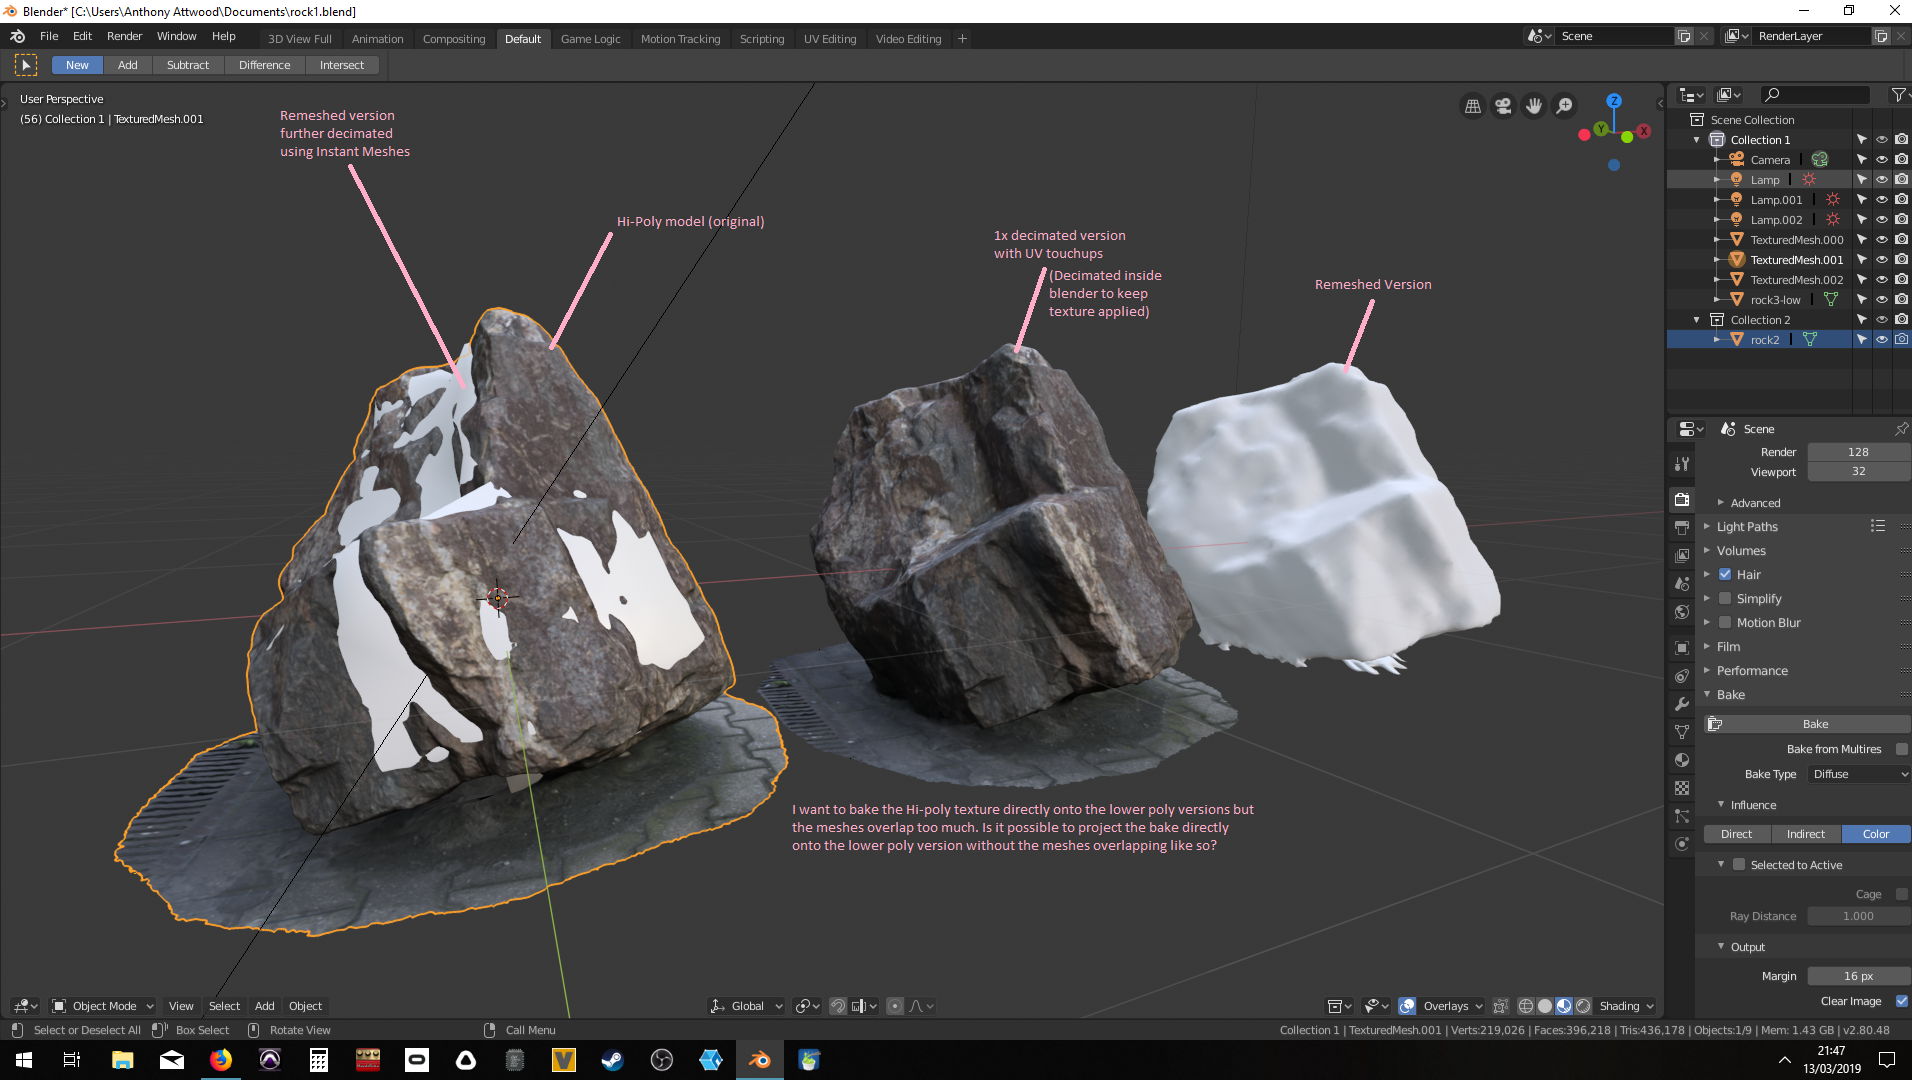
\includegraphics[width = \linewidth]{img/3dsmax_1.png}
    \caption{Baking delle mesh di uno degli oggetti ricreati}
\end{figure}

L'obiettivo \`e quello di effettuare il bake solo nelle alte frequenze della normal map per avere un materiale di dettagli elevati. %paragrafo da ampliare
\\
\\
Per il processo di baking delle texture abbiamo deciso di utilizzare il software "Knald" in quanto \`e veloce e grazie al supporto del formato .ply ci permette pi\`u flessibilit\`a per lavorare su Unity.
Abbiamo anche testato "Substance Designer" ma non abbiamo avuto gli stessi risultati soddisfacenti ottenuti con Knald.

%sostituire immagine
\begin{figure}[H]
    \centering
    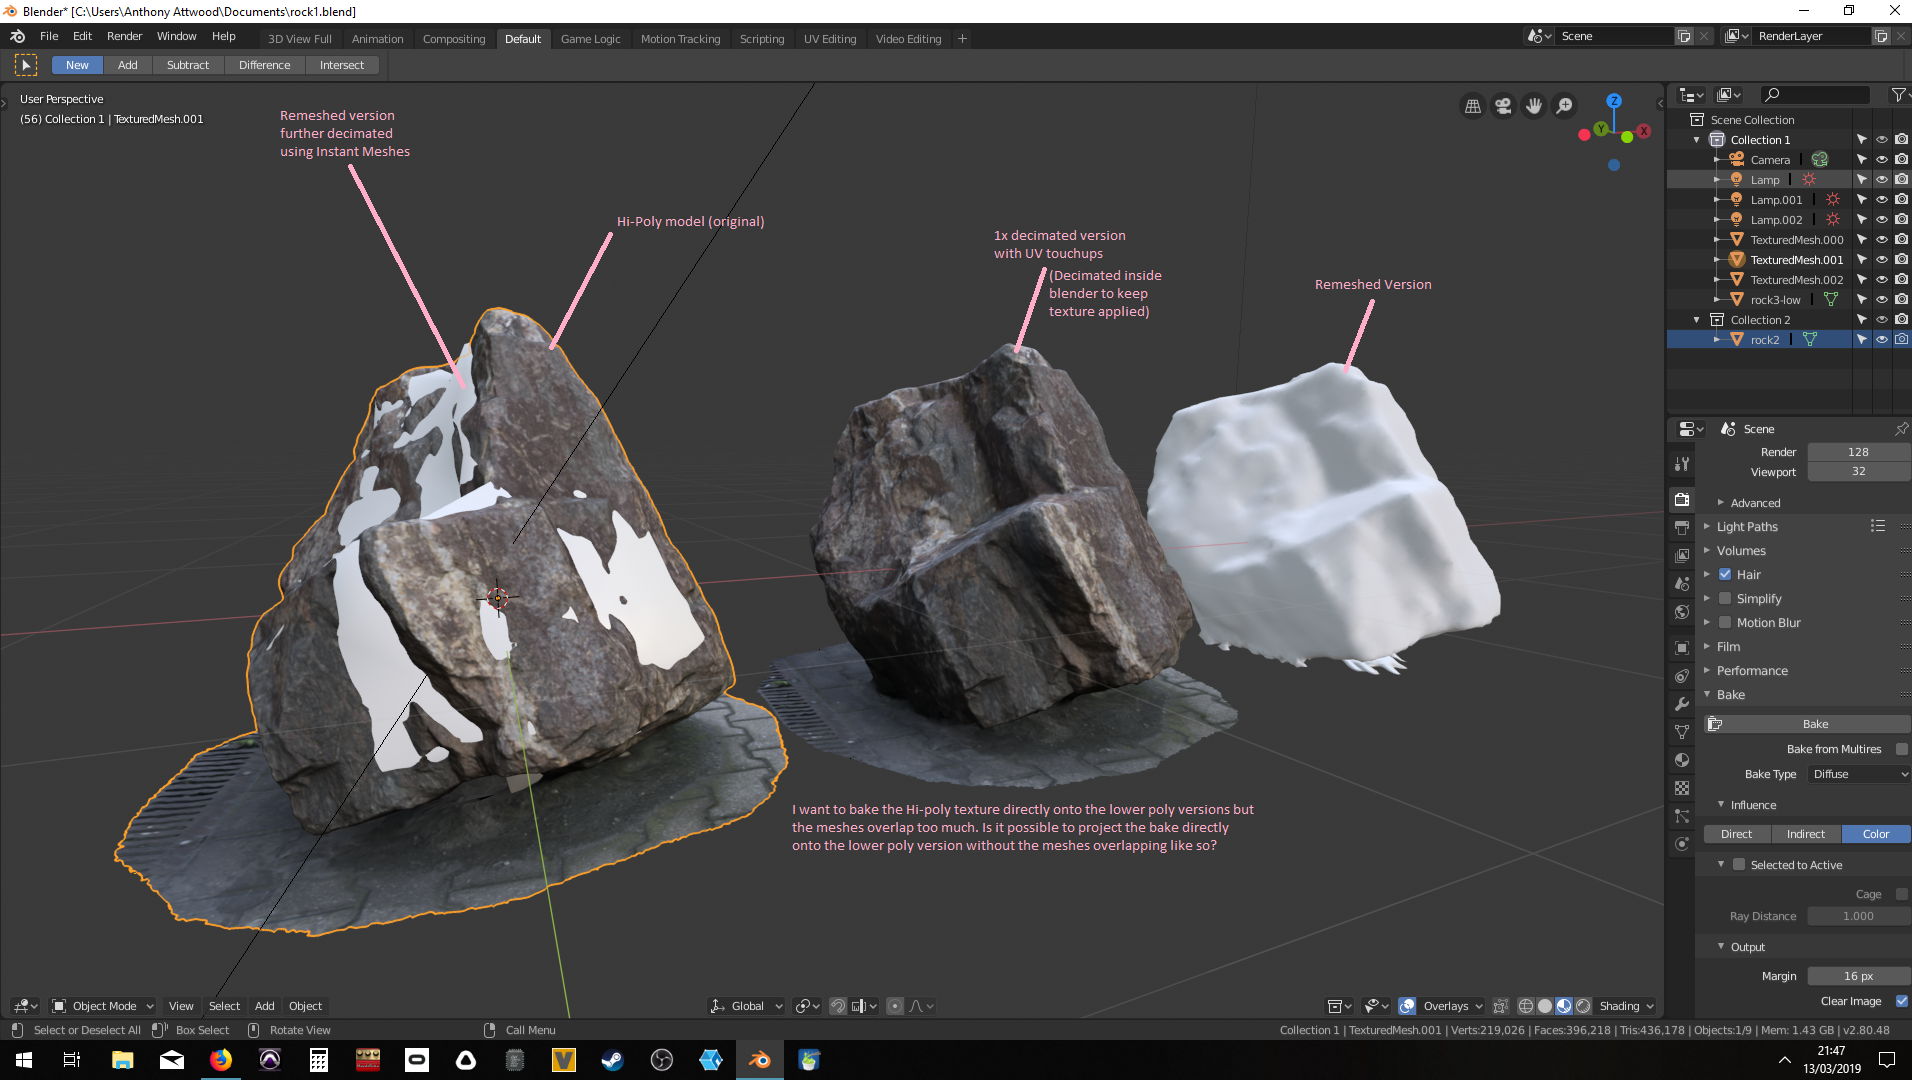
\includegraphics[width = \linewidth]{img/3dsmax_1.png}
    \caption{Baking delle texture grazie al software Knald}
\end{figure}

A questo punto abbiamo rimosso le luci e le ombre eccessive dalle texture. Per questo processo abbiamo utilizzato il software automatico di rimozione delle luci di Unity (Delightning tool). Dato che non avevamo bisogno delle texture ripetibili siamo passati alla finalizzazione e creazione dell'asset pronto per essere importato nella scena di Unity. Per fare ci\`o siamo nuovamente ricorsi al software 3DSMax.

%sostituire immagine
\begin{figure}[H]
    \centering
    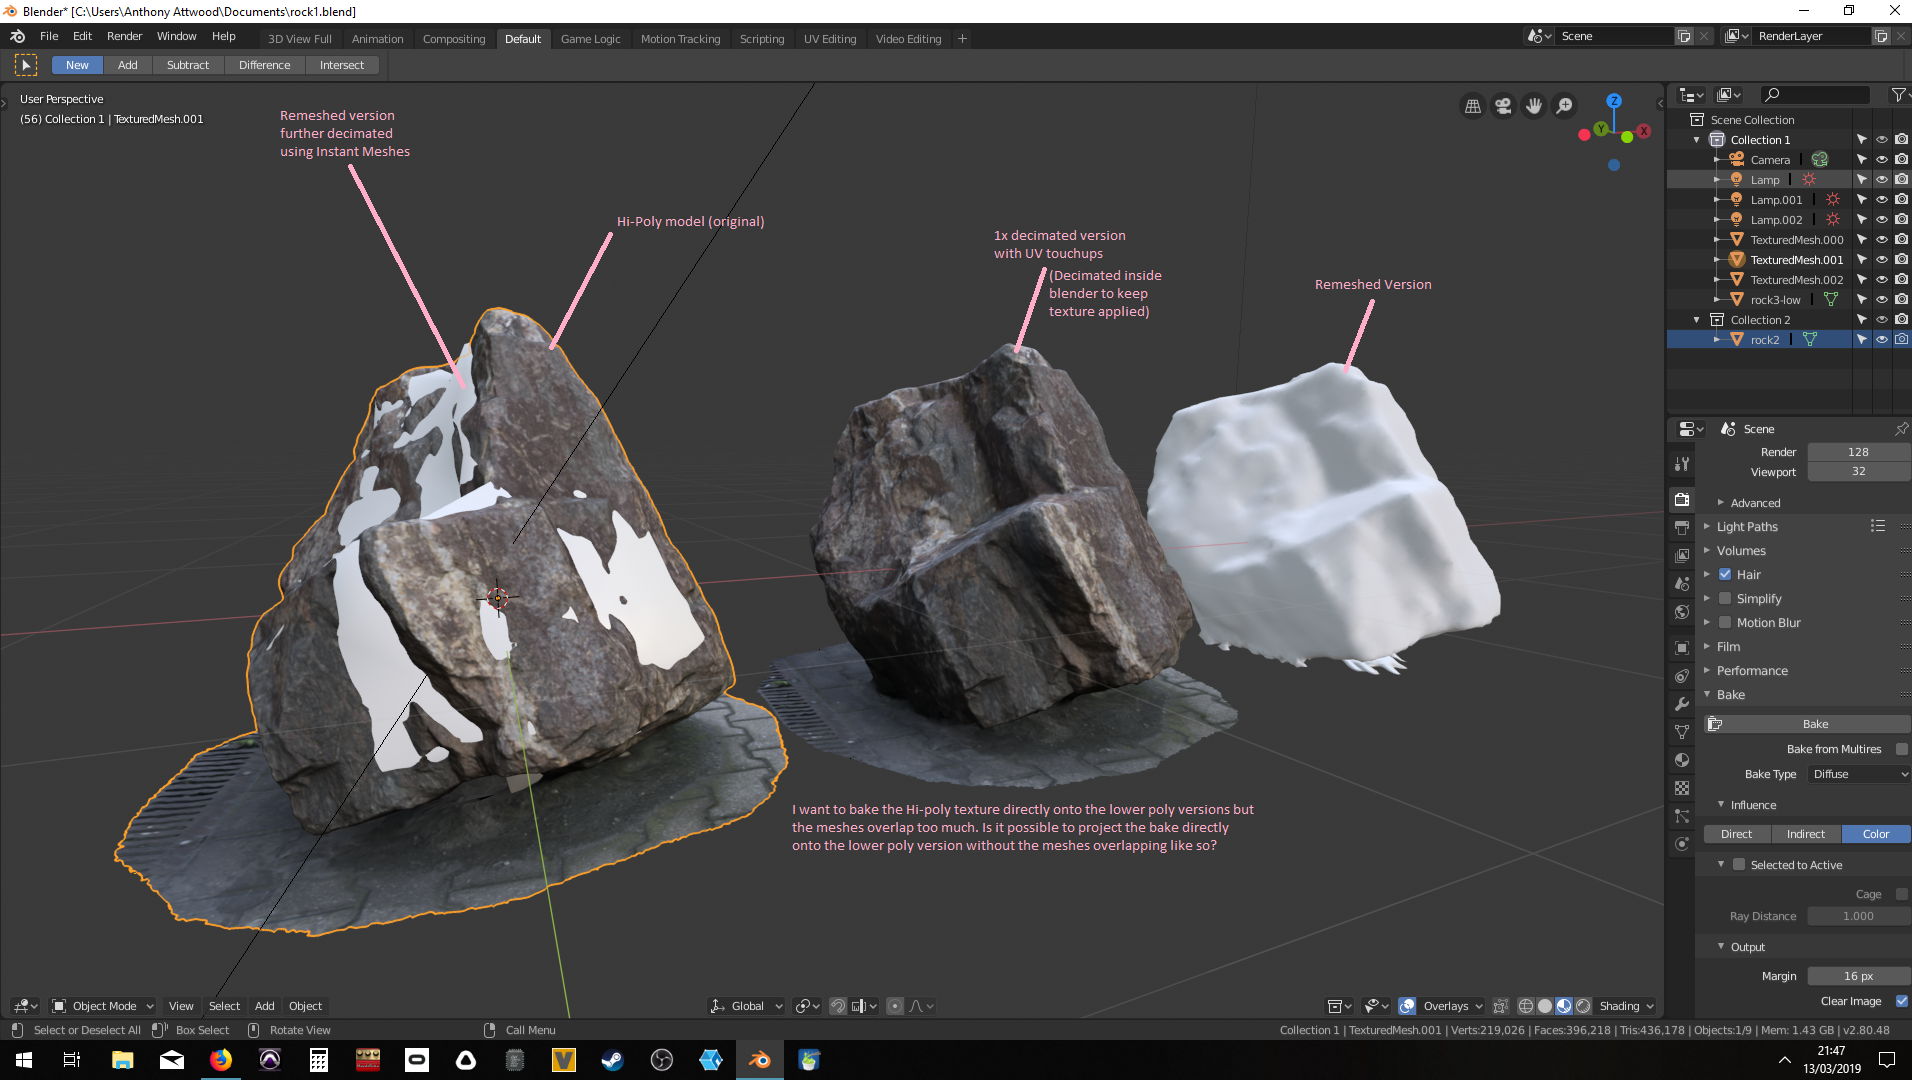
\includegraphics[width = \linewidth]{img/3dsmax_1.png}
    \caption{Finalizzazione dell'Asset}
\end{figure}

\newpage
\subsection{Unity e composizione grafica}
\begin{figure}[H]
    \centering
    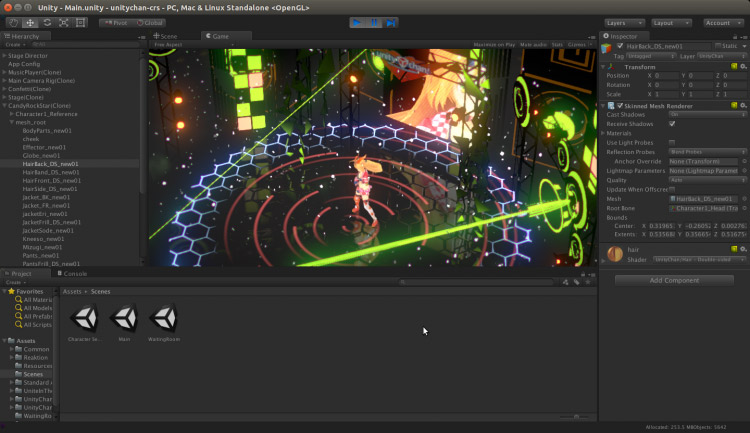
\includegraphics[width = \linewidth]{img/unity-3d-linux.jpg}
    \caption{Una schermata dell'Editor di Unity}
\end{figure}

Per comporre la scena e gli oggetti creati con Zephyr ci siamo affidati al motore grafico pi\`u utilizzato al mondo: \textbf{Unity}

Per apprendere quest'immenso software ci siamo affidati alla documentazione ufficiale (\href{https://docs.unity3d.com/Manual/index.html}{Unity User Manual}) e alla sperimentazione sulle template gratuite create da Unity. (\href{https://assetstore.unity.com/packages/essentials/asset-packs/standard-assets-32351}{Standard Assets}).
Unity permette di creare giochi compatibili su diverse piattaforme dando allo sviluppatore tutti gli strumenti necessari per concentrarsi sulla creazione e non sull'ottimizzazione.

\newpage
\section{Definizione del Progetto}

Il nostro progetto consiste nella creazione di un ambiente virtuale completamente esplorabile e che interagisce a determinate azioni effettuate dal giocatore. Abbiamo inoltre preso un oggetto reale di interesse storico ovvero una statua del Giardino Salvi di Vicenza e con il software Zephyr ne abbiamo riscostruito il modello 3D inserendo l'oggetto all'interno del mondo di gioco.

\subsection{Gameplay}
L'obbiettivo del giocatore \`e quello di:
\begin{itemize}
\item esplorare il vasto mondo di gioco alla ricerca di determinati oggetti
\item utilizzare gli oggetti in una determinata sequenza per raggiungere l'uscita e terminare il gioco
\end{itemize} 

Tutti gli oggetti che il giocatore dovr\`a trovare saranno realizzati con la tecnica della fotogrammetria realizzata grazie al software 3DF Zephyr. 
Il gioco sar\`a composto da vari livelli che seguiranno un progressivo incremento di difficolt\`a, all'inizio il giocatore potr\`a limitarsi all'esplorazione e alla raccolta ma procedendo aumenter\`a il livello di sfida.

\newpage
\subsection{Trama}
La Trama è attualmente in fase di revisione.

%--------GRAFICO---------------
%\begin{center}
%\begin{tikzpicture}
%\begin{axis}[
%    title={Copie vendute di giochi surival horror dal 2000 al 2019},
%    xlabel={Anno},
%    ylabel={Copie vendute [in milioni]},
%    xmin=2000, xmax=2019,
%    ymin=5, ymax=130,
%    xtick={2000,2005,2010,2015,2019},
%    ytick={5,18,46,95,147},
%   ymajorgrids=true,
%   grid style=dashed,
%]
% 
%\addplot[
%    color=red,
%    mark=square,
%   ]
%    coordinates {
%    (2000,6)(2005,17)(2010,34)(2015,65) (2019,127) 
%    };
%    \legend{}
% 
%\end{axis}
%\end{tikzpicture}
%\end{center}

\subsection{Grafica}
Verr\`a utilizzato uno stile grafico fotorealistico che permetter\`a al giocatore una completa immersione all'interno del mondo di gioco, incrementata inoltre dall'utilizzo del VR.
Le ambientazioni saranno costituite da diversi biomi che varieranno a seconda del livello o della zona.


%----------TABELLA GRAFICA----------
%\begin{center}
%{\rowcolors{3}{white!80!white!50}{green!70!white!40}
%\begin{tabular}{ |p{3cm}|p{3cm}|p{3cm}|  }
%\hline
%\multicolumn{3}{|c|}{Requisiti di sitema} \\
%\hline
%Compenente& Minimi & Consigliati \\
%\hline
%CPU & i5-8400 & i9-9900k \\
%GPU & 1060 & 2080 ti \\
%RAM & 4 GB & 16 GB \\
%DirectX & 9.0 & 12.0 \\
%Spazio su disco & 10 GB & 10 GB \\
%OS & Windows 7 & Windows 10   \\
%\hline
%\end{tabular}
%}
%\end{center}

%\chapter{Untitled Game}

\end{document}
%END----------------------------------------------------
